\section{第八章
总结与展望}\label{ux7b2cux516bux7ae0-ux603bux7ed3ux4e0eux5c55ux671b}

\subsection{8.1 工作总结}\label{ux5de5ux4f5cux603bux7ed3}

\subsubsection{8.1.1 研究回顾}\label{ux7814ux7a76ux56deux987e}

本文围绕''通用多智能体 FPGA
设计全流程自动化框架''这一核心论点，设计并实现了一套面向 DAG
可分解多模块硬件设计的通用自动化框架，并以 AES-128
加密全系统作为验证案例进行了端到端的实验验证。该框架以 OpenHands SDK
为运行底座，以 DeepSeek Chat 双 Profile 策略为 LLM 后端，以 Verilator
仿真器为验证引擎，实现了从规格输入到集成验证通过的全流程自动化。

本文所解决的核心问题是：在硬件设计这一高精度、强约束的领域中，如何设计一套通用的自动化框架来驾驭本质上不可靠的大语言模型，使其成为可信赖的设计自动化组件。现有方案（以
AutoGen 方案为典型代表）将控制权交给 LLM
自身，依赖提示词中的自然语言指令约束 Agent
行为；而本文提出并实现的框架控制（Framework-controlled）架构，将批次推进、验证判定、修复决策等控制逻辑全部内化到通用的状态机和
Pydantic 数据契约中，LLM
只负责执行被明确分配的局部任务。这一框架的通用性体现在：其核心架构（编排状态机、分层验证、约束引擎）不依赖于特定的硬件设计对象，AES-128
是其第一个完整的验证案例。

\subsubsection{8.1.2
三个创新点的实现情况}\label{ux4e09ux4e2aux521bux65b0ux70b9ux7684ux5b9eux73b0ux60c5ux51b5}

\begin{figure}
\centering
\pandocbounded{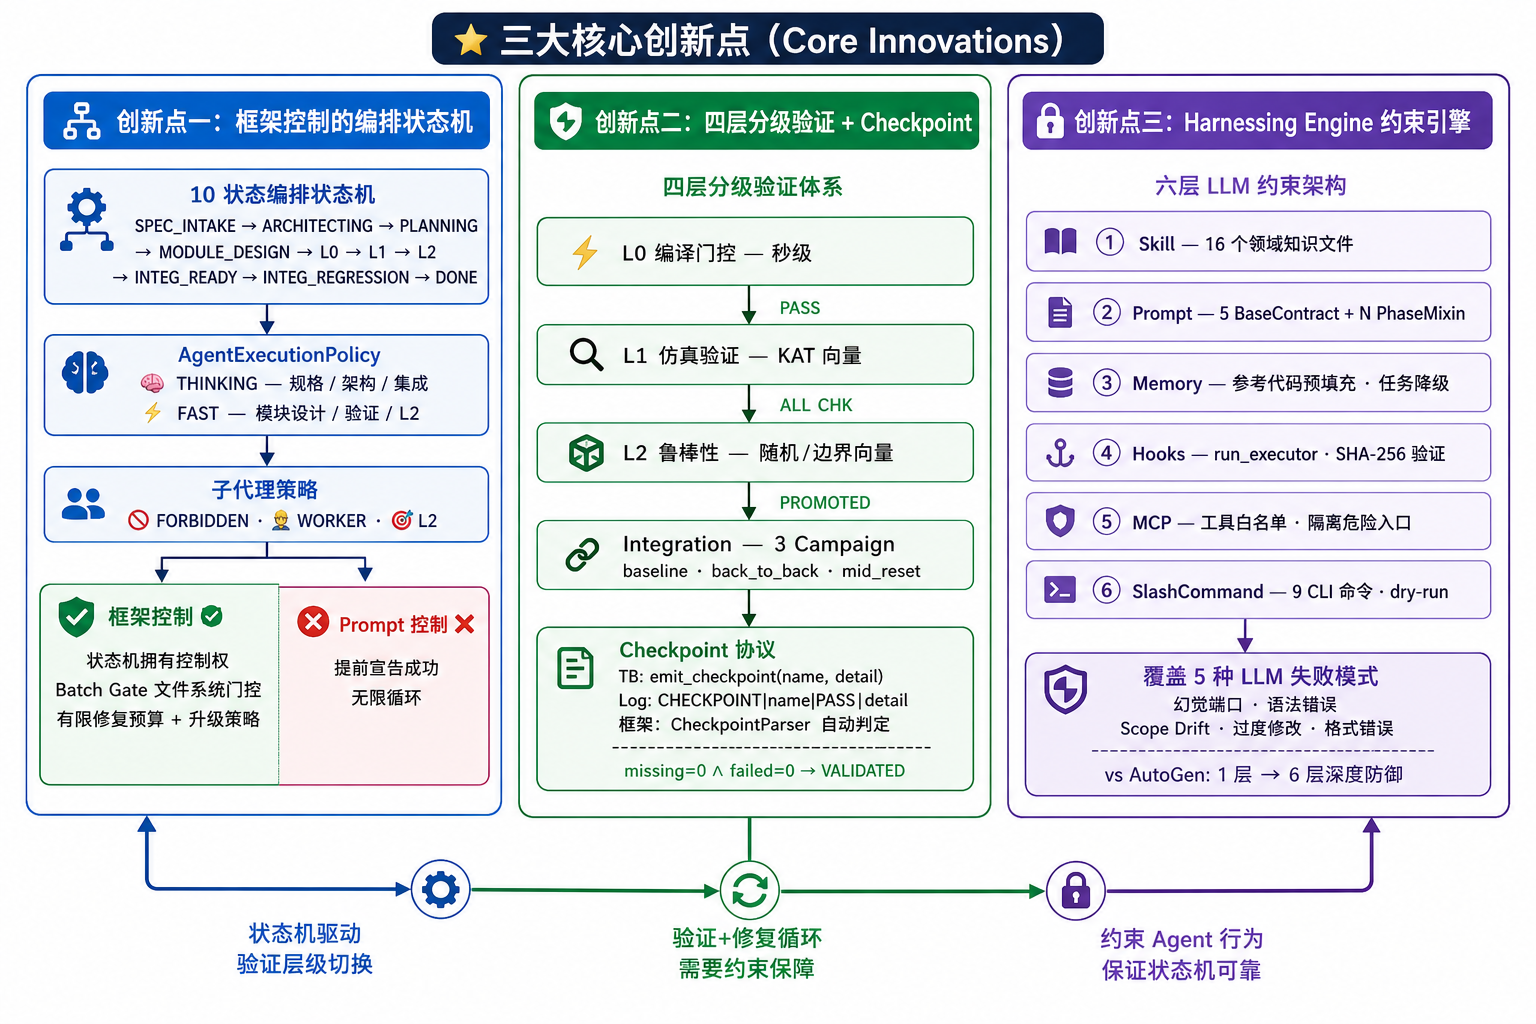
\includegraphics[keepaspectratio,alt={图8-1: 三个核心创新点关系架构}]{../fpga_flow/diagrams/17_core_innovations.png}}
\caption{图8-1: 三个核心创新点关系架构}
\end{figure}

\textbf{创新点一：基于 10 状态编排状态机 + AgentExecutionPolicy
的框架控制多智能体协作架构}

本文提出了一种面向 DAG
可分解多模块硬件设计的通用框架控制架构：编排状态机定义从规格解析到集成验证的全生命周期状态空间，\texttt{AgentExecutionPolicy}
将每个状态映射到确定的 LLM Profile 和
SubagentPolicy，\texttt{DAGBatchPlanner} 基于拓扑排序将任意 DAG
分解为可并行执行的批次层。这一状态机 +
策略的架构模式不依赖于特定的硬件设计对象，可通过替换蓝图函数适配不同的多模块设计任务。

在 AES-128 验证案例中，该状态机实例化为 10
个具体状态（\texttt{SPEC\_INTAKE} → \texttt{ARCHITECTING} →
\texttt{PLANNING} → \texttt{MODULE\_DESIGN} → \texttt{MODULE\_L0} →
\texttt{MODULE\_L1} → \texttt{MODULE\_L2\_OPTIONAL} →
\texttt{INTEGRATION\_READY} → \texttt{INTEGRATION\_REGRESSION} →
\texttt{DONE}），DAGBatchPlanner 将 4 节点 AES DAG
分解为三个执行层，在依赖满足后自动并行执行 Layer 2 的两个模块，这是
AutoGen 线性 pipeline 方案无法实现的能力。该创新点已通过
\texttt{orchestrator/state\_machine.py}、\texttt{policy.py}、\texttt{delegation.py}
等核心模块实现，并在端到端 \texttt{run-aes-mvp} 流程中得到验证。LED
Chaser
案例进一步验证了该状态机在非密码学单模块设计上的完整复用性------同一 10
状态编排状态机驱动了从 SPEC\_INTAKE 到 DONE
的全流程执行，所有状态转移逻辑和 AgentExecutionPolicy
策略映射无需任何修改。

\textbf{创新点二：L0→L1→L2→Integration 四层分级验证体系与 Checkpoint
协议}

该验证体系的架构设计面向通用多模块硬件设计，Checkpoint
协议和分层验证逻辑不依赖于特定设计对象。\texttt{CHECKPOINT\textbar{}\textless{}name\textgreater{}\textbar{}PASS\textbar{}\textless{}detail\textgreater{}}
协议将验证意图精确编码为机器可解析的文本格式，由
\texttt{CheckpointParser} 自动判定，任何硬件设计均可通过定义自身的
Checkpoint 列表接入这一体系。

在 AES-128
验证案例中，本文设计并实现了四层分级验证体系，通过快速失败原则（L0
编译门控在仿真前拦截语法错误）和逐步深入策略（从单向量验证到随机鲁棒测试再到多场景集成回归），覆盖了从语法正确性到系统级行为正确性的完整验证空间。4
个模块共设计了 9 个 Checkpoint（aes\_sbox 1 个，aes\_key\_schedule\_128
1 个，aes\_round\_transform 1 个，aes128\_encrypt\_core 6
个），集成回归测试通过 baseline、back\_to\_back、mid\_reset 三种
Campaign 覆盖了连续加密和异常复位等系统级场景。该创新点通过
\texttt{executors.py} 中的
\texttt{L0Executor}、\texttt{L1Executor}、\texttt{L2CampaignExecutor}、\texttt{IntegrationRegressionExecutor}
四个执行器实现，并通过 \texttt{aes\_tb\_common.hpp} 中的
\texttt{emit\_checkpoint()} 接口与 Testbench 端协同工作。LED Chaser
案例定义了 4 个自定义
Checkpoint（CHK\_RESET\_CLEAR、CHK\_SHIFT\_LEFT、CHK\_SHIFT\_RIGHT、CHK\_WRAP\_AROUND），无需修改框架代码即通过
Checkpoint 协议验证，证明了验证体系的设计无关性。

\textbf{创新点三：Harnessing Engine ---
Skill/Prompt/Memory/Hooks/MCP/SlashCommand 六层约束引擎}

Harnessing Engine 的六层约束架构是一种通用的 LLM
行为约束模式，可通过替换领域内容适配不同的硬件设计目标，甚至扩展到软件工程等其他
LLM 应用场景。其核心洞察是：单一 system\_message 层不足以可靠约束 LLM
在高精度强约束领域中的行为，需要从
Skill、Prompt、Memory、Hooks、MCP、SlashCommand
六个维度形成多层防御矩阵。

在 AES-128 验证案例中，本文提出了 Harnessing Engine
概念，系统性地将对不可靠 LLM 的约束工程从单一 system\_message
层扩展为六层结构化约束组合：Skill 层通过 16 个领域知识文件为 Agent
注入权威规则；Prompt 层通过可组合的 BaseContract + PhaseMixin
架构精确控制每个执行阶段的行为边界；Memory
层将验证通过的参考代码预填充到工作区，显著降低从零生成正确 RTL
的难度；Hooks 层通过 \texttt{run\_executor} 自定义工具和
\texttt{verify\_repair\_edit()} 哈希验证构建执行门控；MCP
层通过工具过滤（排除 \texttt{verilator\_testbenchgenerator} 和
\texttt{verilator\_naturallanguage}）防止 Agent
绕过框架直接生成代码；SlashCommand 层提供完整的 CLI
命令体系，每条命令对应确定的验证语义。六层协同覆盖了幻觉端口、语法错误、Scope
drift、过度修改、格式错误 5 种典型 LLM
失败模式，形成了多维度的防御矩阵。LED Chaser 案例以
\texttt{memory\_required:\ false} 配置运行，验证了 Harnessing Engine
在无 Memory 预填充场景下的有效性------仅依赖
Skill、Prompt、Hooks、MCP、SlashCommand
五层约束即驱动从零生成并验证通过。

\subsubsection{8.1.3
实验验证结论}\label{ux5b9eux9a8cux9a8cux8bc1ux7ed3ux8bba}

实验结果表明，本文提出的框架在 AES-128 加密全系统案例上实现了以下目标：

\begin{itemize}
\tightlist
\item
  全流程可跑通：从 \texttt{run-aes-mvp} 命令启动到状态机到达
  \texttt{DONE} 状态，不需要人工干预；
\item
  模块验证全部首次通过：全部 4
  个模块（aes\_sbox、aes\_key\_schedule\_128、aes\_round\_transform、aes128\_encrypt\_core）均在首次生成后直接通过
  L0 编译与 L1 Checkpoint 验证，修复轮次均为 0，首次通过率 100\%；
\item
  集成回归全部通过：3 个集成
  Campaign（baseline、back\_to\_back、mid\_reset）全部 PASS，6/6
  Checkpoint 通过，验证了 AES-128 全系统在 NIST KAT
  向量、连续多帧加密和异步复位恢复场景下的正确性；
\item
  框架控制有效：16 个批次中 11 个修复批次因
  \texttt{condition\_false}（首次验证已通过）被跳过，所有批次推进决策均由状态机和
  Checkpoint 判定逻辑驱动，LLM 无法绕过验证门控''提前宣布成功''；
\item
  Checkpoint
  协议稳定：\texttt{CHECKPOINT\textbar{}\textless{}name\textgreater{}\textbar{}PASS\textbar{}\textless{}detail\textgreater{}}
  格式在所有模块的仿真日志解析中稳定工作，\texttt{CheckpointParser}
  能从含有其他调试输出的日志中准确提取 Checkpoint 行；
\item
  跨设计通用性实证：LED Chaser（4 位 LED 流水灯）案例通过 YAML
  蓝图驱动机制（\texttt{run-design\ -\/-blueprint}），在不修改任何框架代码的前提下完成了从规格输入到集成验证通过的全流程执行，4/4
  自定义 Checkpoint 全部通过，修复轮次为 0，Workflow gate 判定为
  success，实证了框架的跨设计通用性；
\item
  FPGA 工具链端到端验证：通过编写 Vivado
  自动化脚本，将系统输出的 RTL/TB 代码自动调用 Xilinx Vivado
  完成仿真波形生成、逻辑综合、布局布线和比特流编译全流程，AES-128 和 LED
  Chaser 两个设计均成功生成 \texttt{.bit} 文件，综合无错误、时序无违例，实现了从
  AI 生成代码到硬件可运行产物的完整闭环。
\end{itemize}

本文的工作相比 AutoGen 方案，实现了从线性 pipeline 到 DAG
拓扑批调度、从单层验证到四层分级验证、从 Prompt-controlled 到
Framework-controlled
的系统性架构升级。这些架构升级在设计层面是通用的，AES-128 全系统和 LED
Chaser
双案例的成功验证证明了该通用框架在不同设计实例上的有效性，为多智能体
FPGA 设计自动化的可靠性与可扩展性研究提供了一个完整的工程实践参考。

\begin{center}\rule{0.5\linewidth}{0.5pt}\end{center}

\subsection{8.2 不足与展望}\label{ux4e0dux8db3ux4e0eux5c55ux671b}

\subsubsection{8.2.1 当前局限}\label{ux5f53ux524dux5c40ux9650}

尽管本文在 AES-128
案例上完整验证了框架设计，但当前版本仍存在以下明确局限：

\textbf{局限一：设计覆盖范围有限，多模块非密码学设计尚未验证}。本框架已通过
YAML 蓝图驱动机制（\texttt{BlueprintLoader} +
\texttt{run-design\ -\/-blueprint}）实现了声明式的零代码适配能力，LED
Chaser
案例验证了该机制的有效性。然而，当前仅覆盖两个验证案例：AES-128（多模块密码学设计）和
LED Chaser（单模块数字逻辑设计）。框架尚未在多模块非密码学设计（如 FIFO
+ AXI 总线接口组合、浮点运算管线等）上进行验证，DAG 拓扑批调度在非 AES
的多模块设计上的表现仍待实证。此外，\texttt{\_aes\_blueprints()}
硬编码函数仍作为 AES-128 的快捷路径保留在 \texttt{synthesis.py} 中，YAML
蓝图路径已成为推荐的通用适配方式。

\textbf{局限二：L3 综合与实现阶段尚未深度集成到框架}。本文通过编写 Vivado
自动化脚本实现了从系统输出的 RTL/TB 代码到比特流生成的离线全流程验证（详见
§7.7），确认了生成代码的可综合性与时序收敛性。然而，当前 Vivado
脚本作为独立工具运行在框架状态机的 \texttt{DONE}
状态之后，尚未集成到框架的分层验证体系中------框架无法自动解读综合报告中的时序违例信息并指导
RTL 修改，也不具备根据资源利用率报告自动优化设计的能力。因此，当前框架尚不能替代完整的
FPGA 实现流程中的自动化闭环。

\textbf{局限三：依赖 DeepSeek API，存在外部依赖}。全流程依赖
\texttt{DEEPSEEK\_API\_KEY} 和 DeepSeek 官方 API
端点（\texttt{https://api.deepseek.com}），网络延迟、API
限流和服务可用性均可能影响自动化流程的稳定性。在受限网络环境（如企业内网）中部署存在障碍。

\textbf{局限四：Memory 预填充依赖已有参考代码}。\texttt{MemoryStore}
的工作前提是 Skill 文件中已经存在验证通过的参考 RTL 和
Testbench。对于全新的未见过的硬件设计模块，框架目前没有自主从零构建参考代码库的机制------这意味着框架的有效性在一定程度上依赖于人工维护的技能文件库。

\textbf{局限五：仅在单机单用户场景验证}。当前框架在 macOS
单机环境下验证，未测试分布式执行、多用户并发或 CI/CD
流水线集成场景的稳定性。

\subsubsection{8.2.2 未来方向}\label{ux672aux6765ux65b9ux5411}

基于上述局限，本文提出以下五个未来研究方向：

\textbf{方向一：扩展至多模块非密码学设计}。LED Chaser 案例已验证了 YAML
蓝图驱动的声明式适配机制在单模块设计上的有效性，下一步的优先验证目标是多模块非密码学设计------如
FIFO + AXI 总线接口组合、浮点运算管线、SPI/I2C 控制器等，以验证 DAG
拓扑批调度和多模块并行执行在更广泛的硬件设计领域中的通用性。同时，密码学方向可扩展至
AES-192/AES-256、SHA-256、RSA
等模块，验证蓝图驱动机制在不同复杂度的密码学设计上的适用性。

\textbf{方向二：将 L3 综合与实现阶段深度集成到框架}。本文已通过 Vivado
自动化脚本实现了离线的综合、布局布线和比特流生成验证（详见 §7.7），证明了生成代码在真实
FPGA 工具链上的可实现性。下一步是将该脚本升级为框架的正式 L3
验证层：设计 \texttt{VivadoMCPAdapter}（类似现有的
\texttt{VerilatorMCPAdapter}），将综合、实现和比特流生成封装为 MCP
工具调用；开发结构化的综合报告解析器，自动提取时序违例（WNS/WHS）和资源利用率信息；实现
\texttt{L3Executor}
执行器，将综合结果反馈给 Agent 以指导 RTL 优化，形成
L0→L1→L2→L3→Integration 的五层完整验证闭环。这将使框架从''生成代码并验证功能正确性''进一步升级为''生成代码并保证硬件可实现性''。

\textbf{方向三：支持多 LLM 后端}。当前框架深度绑定 DeepSeek Chat
API，通过扩展 \texttt{LLMProfileName} 枚举和
\texttt{build\_llm\_profile\_kwargs()} 函数，引入对
Claude（Anthropic）、GPT-4o（OpenAI）和本地部署的 Llama-3/Qwen
等模型的支持，使用户可以根据网络环境、成本预算和性能需求灵活选择 LLM
后端。同时，可以探索混合 LLM
策略：对于编排器使用最强模型，对于工作器使用成本效益比更高的本地模型，进一步降低运行成本。

\textbf{方向四：Agent 自主学习能力}。当前 Memory
预填充依赖人工维护的静态 Skill
文件。未来可以设计基于修复历史的自主学习机制：每次成功的修复循环（RepairContract
→ EditReceipt → VALIDATED）自动触发一次 Skill
更新流程，将修复前后的代码差异（diff）和修复原因（RepairContract
描述）结构化写入对应的 Skill
文件，形成动态增长的领域知识库。经过多次运行后，框架对同类错误的首次通过率将逐步提升，修复轮次逐步减少。

\textbf{方向五：Harnessing Engine 的通用化框架}。本文的 Harnessing
Engine 已在架构层面以通用性为目标设计，其六层约束架构（Skill / Prompt /
Memory / Hooks / MCP /
SlashCommand）具有超越硬件设计领域的通用价值。未来可以将 Harnessing
Engine
抽象为独立的开源框架库，使其能够以声明式配置的方式应用于软件工程、数据分析、文档生成等不同
LLM 应用场景，为''如何系统性地驾驭不可靠
LLM''这一广泛问题提供可复用的工程模式。

\subsubsection{8.2.3 结语}\label{ux7ed3ux8bed}

FPGA 设计自动化与大语言模型的结合处于研究早期，从''LLM 能否生成正确的
RTL''到''如何构建通用的可靠全流程自动化框架''是一个质的跨越。本文的工作表明，通过精心设计的通用框架控制架构、分层验证体系和多层约束引擎，不可靠的
LLM 可以被驾驭为可信赖的 FPGA 设计自动化组件。AES-128 加密全系统和 LED
Chaser
流水灯双案例的成功验证，从多模块密码学设计和单模块数字逻辑设计两个维度证明了该通用框架的有效性与跨设计适配能力。将这一框架进一步扩展到更复杂的多模块非密码学设计------从通信
IP 核到信号处理单元到总线控制器------并最终缩短从规格到可综合 RTL
的端到端设计周期，是值得持续探索的方向。
